\documentclass[a4paper,12pt, oneside]{article}
\title{Progetto di High Performance Computing}
\author{Gabos Norbert 0000970451}
\date{\today}

\usepackage[T1]{fontenc}
\usepackage[utf8]{inputenc}
\usepackage[italian]{babel}
\pagestyle{plain}
\usepackage{graphicx}
\graphicspath{{images/}}

\begin{document}

\maketitle

\section{Introduzione}

Il programma SPH è un simulatore che si occupa di modellare il comportamento dei fluidi in un
ambiente virtuale. È stato scritto in linguaggio C e progettato per funzionare su un singolo
processore. Per realizzare le versioni parallele del programma, è stato necessario analizzare
la versione sequenziale, al fine di individuare le parti del codice che possono essere eseguite
in parallelo. Le sezioni successive presentano le diverse versioni del programma, con le
relative modifiche e le performance ottenute grazie all'utilizzo di OpenMP e MPI.

\section{Versione OpenMP}

Per creare la versione OpenMP, si è partiti dalla versione sequenziale analizzando il codice.
Una volta individuati i punti da parallelizzare, si sono analizzate eventuali loop carry
dependencies, e si è scoperto che tutti i cicli erano embarrassingly parallel. Si è partiti
dalla funzione più semplice da parallelizzare, ovvero "integrate", in quanto consiste in un
singolo ciclo. Le funzioni compute\_density\_pressure e compute\_forces contengono al loro
interno due cicli annidati, quindi hanno richiesto un po' più di attenzione.
Per la funzione "compute\_density\_pressure", l'intento era quello di parallelizzare entrambi
i cicli mediante la clausola "collapse(2)", però i due cicli sono dipendenti uno dall'altro,
quindi si è deciso di parallelizzare solo il ciclo esterno. Per la funzione "compute\_forces",
l'approccio è stato quello di parallelizzare il ciclo interno, eseguendo una "reduce" sulle
variabili fpress\_x, fpress\_y, fvisc\_x e fvisc\_y. Questa soluzione, purtroppo, è stata
scartata in quanto non ha portato ad un miglioramento delle prestazioni.
Infine, per la funzione "avg\_velocities", si è deciso di utilizzare la funzione reduce sulla
variabile "result" per ottenere il risultato finale.

\section{Versione MPI}

Durante l'inizializzazione della versione MPI, è stata impiegata la funzione Bcast per
distribuire le informazioni relative alle particelle tra i processori. Inoltre, è stato
creato il tipo di variabile "MPI\_PARTICLE" per facilitare l'invio e la ricezione delle
particelle tra i processori.
L'approccio adottato per parallelizzare le varie funzioni ha previsto che ogni processo
avesse le stesse particelle sia all'inizio che alla fine della funzione. A tal fine, è
stata creata la funzione "sync\_particles" che, mediante l'utilizzo di "MPI\_Allgatherv",
permette di raccogliere i dati delle particelle sparse su tutti i processori e di
riorganizzarli in modo che ogni processo abbia le stesse particelle. La funzione
"sync\_particles" viene richiamata alla fine di ogni funzione che modifica le particelle.

Per parallelizzare le funzioni si è diviso l'array in chunk e ogni processo ha eseguito
solamente il proprio chunk. Per quanto riguarda la funzione "avg\_velocities", è stata
utilizzata la funzione "reduce" per ottenere il risultato finale e salvarlo tra tutti i
processi. Questa soluzione avrebbe potuto essere implementata anche attraverso l'uso
della funzione "MPI\_Reduce", ma si è scelto di impiegare "MPI\_Allreduce" per avere 
una soluzione più generale.
Inoltre, alla fine di ogni ciclo, viene richiamata la funzione MPI\_Barrier per garantire
la sincronizzazione tra i processi, anche se questa precauzione potrebbe non essere
strettamente necessaria.

\section{Prestazioni}

\begin{figure}[h]
    \centering
    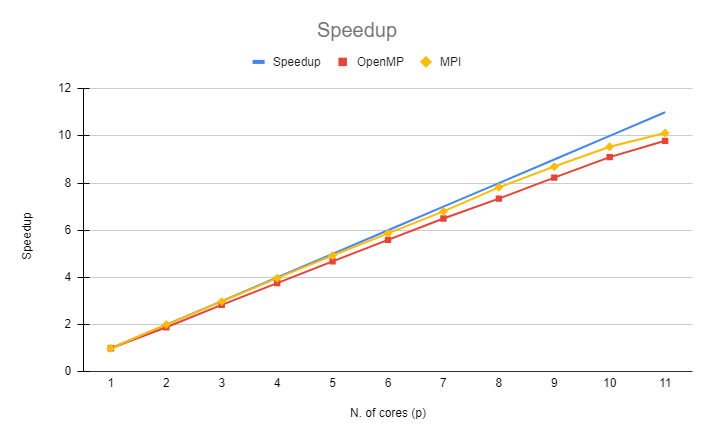
\includegraphics[width=0.75\textwidth]{speedup.png}
    \caption{Speedup}
    \label{fig:speedup}
\end{figure}

\begin{figure}[h]
    \centering
    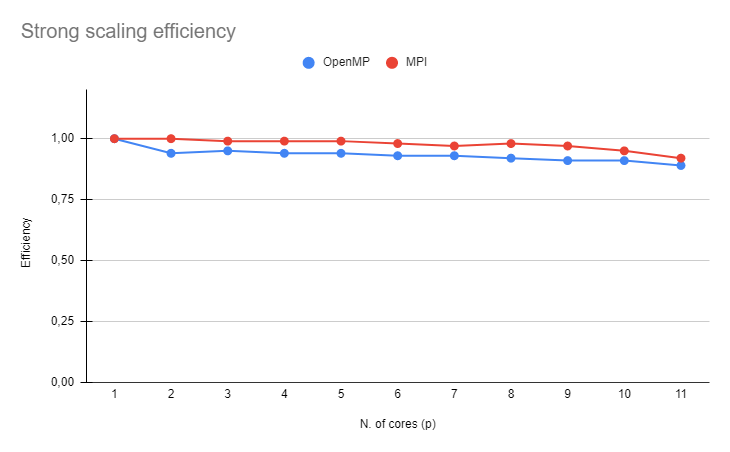
\includegraphics[width=0.75\textwidth]{strong-scaling.png}
    \caption{Strong Scaling Efficiency}
    \label{fig:strong-scaling}
\end{figure}

\begin{figure}[h]
    \centering
    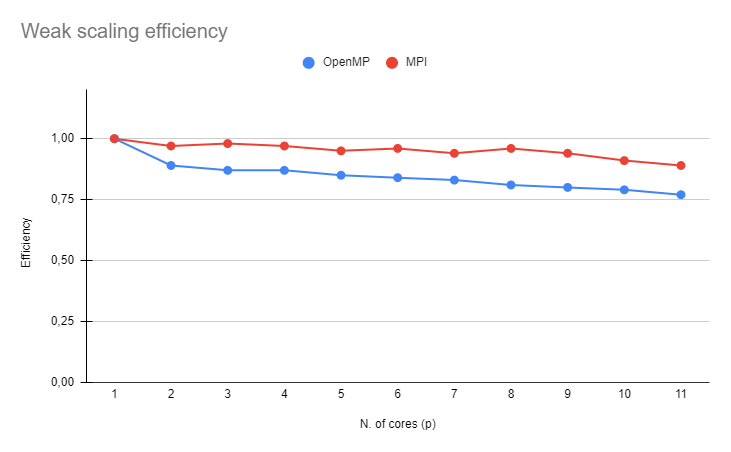
\includegraphics[width=0.75\textwidth]{weak-scaling.png}
    \caption{Weak Scaling Efficiency}
    \label{fig:weak-scaling}
\end{figure}

Nella Figura \ref{fig:speedup}, si può osservare il grafico del speedup ottenuto attraverso
le diverse versioni del programma. È interessante notare come la versione MPI abbia
conseguito un speedup superiore rispetto alla versione OpenMP. Tuttavia, la differenza non
è particolarmente marcata, con un valore medio del 4,71\%.

Nella Figura \ref{fig:strong-scaling}, è possibile osservare l'andamento dell'efficienza di
strong scaling per entrambe le versioni del programma. Analogamente, la Figura \ref{fig:weak-scaling}
illustra l'efficienza di weak scaling per OpenMP e MPI. L'analisi di queste due figure
permette di avere una visione più completa e dettagliata delle prestazioni ottenute
utilizzando le due diverse implementazioni del programma e di comprendere meglio le loro
caratteristiche in termini di scalabilità. Questo ulteriore confronto conferma l'efficacia
della versione MPI nel garantire una maggiore scalabilità e un migliore utilizzo delle
risorse disponibili rispetto all'implementazione basata su OpenMP.

È importante sottolineare che, nonostante il PC utilizzato disponga di 12 core, le
misurazioni sono state effettuate utilizzando solamente 11 core. Questa scelta è stata
fatta perché, utilizzando tutti i 12 core, le prestazioni del programma peggioravano a
causa di altri processi in esecuzione che richiedevano risorse di sistema.

\end{document}
